\documentclass[lettersize, journal]{IEEEtran}
\usepackage[utf8]{inputenc} 
\usepackage[T1]{fontenc}   
\usepackage{mathptmx}       
\usepackage{graphicx}      
\usepackage{float}          
\usepackage{algorithmic}
\usepackage{algorithm}
\usepackage{caption}        
\usepackage{subcaption}     
\usepackage{biblatex}       
\usepackage{amsmath, amsfonts, amssymb}  
\usepackage{hyperref}
\usepackage{enumitem}       
\usepackage{tikz, pgfplots}
\usetikzlibrary{shapes,arrows.meta, positioning}

\addbibresource{reference.bib} 



\begin{document}

% Paper title
\title{Hsopitalisation modelling: A UK Case Study}
\author{Michael Ajao-olarinoye}

\maketitle
% \thispagestyle{empty}


\begin{abstract}

\end{abstract}

\begin{IEEEkeywords}

\end{IEEEkeywords}

\section{Introduction}
\IEEEPARstart{T}{his} introduce your topic and the purpose of your paper.
\section{Problem Statement}

The outbreak of the COVID-19 pandemic has posed significant challenges to healthcare systems worldwide. One of the major concerns during the pandemic's peaks has been the potential overwhelming demand on healthcare resources, particularly the demand for intensive care units (ICUs) and mechanical ventilators. This study aims to develop a mathematical model to understand the dynamics of COVID-19 transmission and forecast the demand for mechanical ventilators in England.

\section{Model Assumptions}

\begin{enumerate}
    \item The population is constant, i.e., no births or non-COVID-related deaths are considered.
    \item The disease transmission occurs only between the susceptible and the infected (both asymptomatic and symptomatic) individuals.
    \item Individuals progress from being exposed to the virus to being infected (either asymptomatic or symptomatic).
    \item Symptomatic infected individuals may require mechanical ventilation if their condition deteriorates.
    \item Ventilated patients either recover or die.
    \item Recovered individuals can lose immunity and become susceptible again.
\end{enumerate}

\section{Model Definition}

\subsection{Compartments}

\begin{itemize}
    \item \( S(t) \): Susceptible individuals at time \( t \).
    \item \( E(t) \): Exposed individuals at time \( t \).
    \item \( I_a(t) \): Asymptomatic infected individuals at time \( t \).
    \item \( I_s(t) \): Symptomatic infected individuals at time \( t \).
    \item \( V(t) \): Individuals on ventilators at time \( t \).
    \item \( R(t) \): Recovered individuals at time \( t \).
    \item \( D(t) \): Deceased individuals at time \( t \).
\end{itemize}

\subsection{Differential Equations}

\begin{align*}
\frac{dS}{dt} & = -\beta S (I_a + I_s) + \omega R \\
\frac{dE}{dt} & = \beta S (I_a + I_s) - \sigma E \\
\frac{dI_a}{dt} & = p \sigma E - \gamma_a I_a \\
\frac{dI_s}{dt} & = (1-p) \sigma E - \gamma_s I_s - \rho I_s \\
\frac{dV}{dt} & = \rho I_s - (\nu + \alpha) V \\
\frac{dR}{dt} & = \gamma_a I_a + \gamma_s I_s + (1-\delta) \alpha V - \omega R \\
\frac{dD}{dt} & = \delta \alpha V + \nu V
\end{align*}

\subsection{Parameters}

\begin{itemize}
    \item \( \beta \): Transmission rate.
    \item \( \sigma \): Rate of progression from exposed to infected.
    \item \( \gamma_a \): Recovery rate for asymptomatic individuals.
    \item \( \gamma_s \): Recovery rate for symptomatic individuals.
    \item \( \rho \): Rate at which symptomatic individuals require ventilation.
    \item \( \alpha \): Recovery rate for ventilated individuals.
    \item \( \nu \): Death rate for individuals on ventilators.
    \item \( \delta \): Proportion of ventilated patients who die.
    \item \( \omega \): Rate at which recovered individuals lose immunity.
    \item \( p \): Proportion of exposed individuals who become asymptomatic infected.
\end{itemize}

\section{Mathematical Proof of the Model}

The above model is a system of ordinary differential equations (ODEs) derived from the law of mass action. The sum of all compartments at any time \( t \) is equal to the constant population \( N \), which ensures the conservation of mass:

\[
S(t) + E(t) + I_a(t) + I_s(t) + V(t) + R(t) + D(t) = N
\]

The non-negativity of the solutions is ensured by the non-negative initial conditions and the fact that the right-hand side of the ODEs does not allow for negative values in any compartment. 

Furthermore, the model's structure ensures that individuals flow through the compartments in a manner consistent with the natural progression of the disease, from exposure to possible death or recovery. The flow is regulated by the parameters, which are all non-negative, ensuring that the transitions between compartments are biologically meaningful.

\section{Real-World Application}

This model serves as a tool for understanding and predicting the demand for critical healthcare resources, specifically mechanical ventilators, in England during the COVID-19 pandemic. By calibrating the model to real-world data, healthcare planners and policymakers can make informed decisions about resource allocation, anticipate periods of high demand, and implement interventions to manage and mitigate the strain on the healthcare system.


\begin{figure}[h]
    \centering
    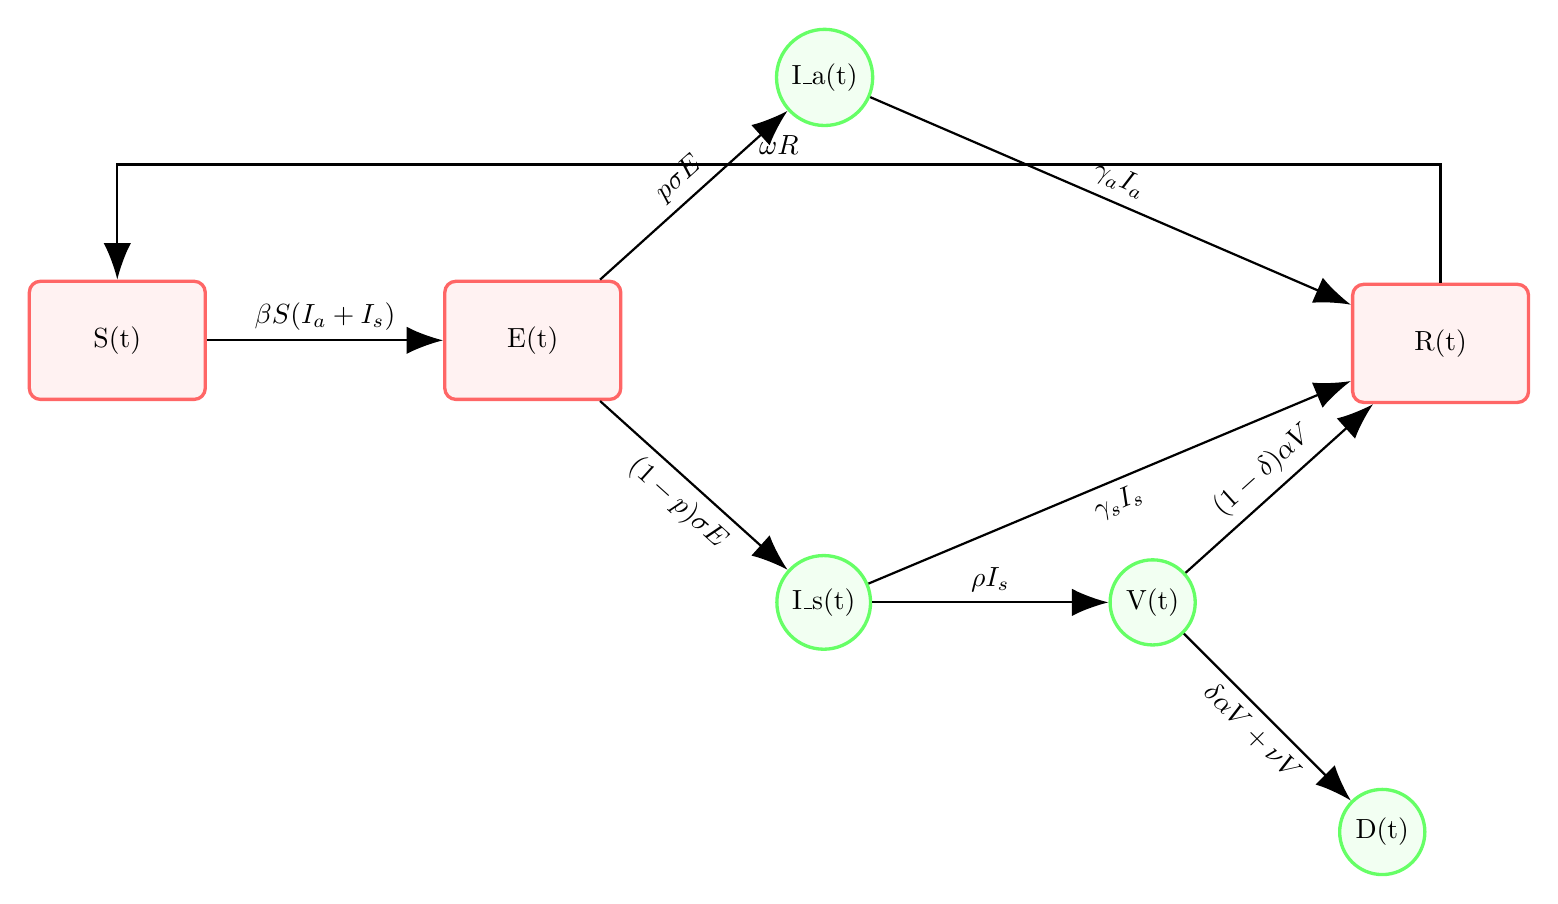
\begin{tikzpicture}[node distance=3cm, auto, thick]
        % Define block styles
        \tikzstyle{roundnode} = [circle, draw=green!60, fill=green!5, very thick, minimum size=7mm, text centered]
        \tikzstyle{squarednode} = [rectangle, draw=red!60, fill=red!5, very thick, text width=2cm, text centered, rounded corners, minimum height=1.5cm]
        \tikzstyle{line} = [draw, -{Latex[scale=2]}]
    
        % Define nodes
        \node [squarednode] (S) {S(t)};
        \node [squarednode, right=of S] (E) {E(t)};
        \node [roundnode, above right=of E] (Ia) {I\_a(t)};
        \node [roundnode, below right=of E] (Is) {I\_s(t)};
        \node [roundnode, right=of Is] (V) {V(t)};
        \node [squarednode, above right=of V] (R) {R(t)};
        \node [roundnode, below right=of V] (D) {D(t)};
        
        % Connect nodes with paths
        \draw[line] (S) -- node[midway, above] { \( \beta S (I_a + I_s) \) } (E);
        \draw[line] (E) -- node[midway, sloped, above] { \( p \sigma E \) } (Ia);
        \draw[line] (E) -- node[midway, sloped, below] { \( (1-p) \sigma E \) } (Is);
        \draw[line] (Is) -- node[midway, above] { \( \rho I_s \) } (V);
        \draw[line] (Ia) -- node[midway, sloped, above] { \( \gamma_a I_a \) } (R);
        \draw[line] (Is) -- node[midway, sloped, below] { \( \gamma_s I_s \) } (R);
        \draw[line] (V) -- node[midway, sloped, above] { \( (1-\delta) \alpha V \) } (R);
        \draw[line] (V) -- node[midway, sloped, below] { \( \delta \alpha V + \nu V \) } (D);
        \draw[line] (R.north) -- ++(0,1.5cm) -| node[pos=0.25, above] { \( \omega R \) } (S.north);
        
    \end{tikzpicture}
    \caption{Compartmental flow of the refined SEIASVHRD model.}
\end{figure}

\end{document}